% !TeX program = lualatex
% !BIB program = biber
% Lualatex is important to render TTF fonts; with pdflatex it's just the regular one
% ratio 16:9 -- https://tex.stackexchange.com/questions/14336/

% compile two versions, inspired by https://tex.stackexchange.com/a/1501
% use the script "compile-pdf.sh"
\newif\ifhandout
% if flags.tex does not exist, create an empty file to be able to compile in TeXstudio
\input{flags}

\ifhandout
\documentclass[12pt,aspectratio=169,handout]{beamer}
\else
\documentclass[12pt,aspectratio=169]{beamer}
\fi



% TODO change "leftfootertext" to your liking
\newcommand{\leftfootertext}{\insertsubtitle}  % just the \title{} text by default
%\newcommand{\leftfootertext}{RNNs and encoder-decoder architectures}  % Your name, for instance


% ------- RUB specifics ----------
% adjust for 16:9
% https://tex.stackexchange.com/questions/354022/modifying-the-margins-of-all-slides-in-beamer
\setbeamersize{text margin left=0.3cm,text margin right=4.5cm} 


% use Metropolis as the basis theme
\usetheme[subsectionpage=progressbar]{metropolis}
% blocks with background globally
\metroset{block=fill}


\usepackage{fontspec}
% RUB fonts need to be installed
% 'UprightFont = * Light' makes sure that the base font is RubFlama Light, which looks
% lighter than RubFlama Regular (would be too thick for slides)
\setsansfont[Scale=MatchLowercase, UprightFont = * Light, BoldFont = * Bold]{RubFlama}
%\setsansfont{Arial} % Open source alternative if you don't have RubFlama

% RUB color scheme
% Dark blue: 0; 53; 96; #003560
\definecolor{RUBDarkBlue}{RGB}{0, 53, 96}

% Light yellow (table fill, etc.); 238; 250; 196; #EEFAC4
\definecolor{RUBLightYellow}{RGB}{238, 250, 196}

%Light green: 141; 174; 16
\definecolor{RUBLightGreen}{RGB}{141, 174, 16}


\setbeamercolor{titlelike}{fg=RUBDarkBlue}
\setbeamercolor{subtitle}{fg=RUBLightGreen}
\setbeamercolor{separation line}{fg=RUBLightGreen}
\setbeamercolor{frametitle}{bg=white, fg=RUBDarkBlue}

% horizontal line on title page and sections
\setbeamercolor{alerted text}{fg=RUBLightGreen}


% Adjust footer bottom (too large by default)
\setbeamertemplate{footline}{%
  \begin{beamercolorbox}[wd=\textwidth, sep=2ex]{footline}%
    \usebeamerfont{page number in head/foot}%
    \usebeamertemplate*{frame footer}
    \hfill%
    \usebeamertemplate*{frame numbering}
  \end{beamercolorbox}%
}


% Lab name, numbering, etc. in footer
\setbeamertemplate{frame numbering}{TrustHLT --- Prof.\ Dr.\ Ivan Habernal \hspace*{1ex} 
\includegraphics[width=7em]{img/rub-logo.pdf}\hspace*{1ex}}

\setbeamertemplate{frame footer}{\hspace*{1ex}\insertframenumber \hspace*{2ex} \leftfootertext}

% adjust the background to be completely white
\setbeamercolor{background canvas}{bg=white}

% logos on the title page
\titlegraphic{%
	\begin{picture}(0,0)
		\put(435,0){\makebox(0,0)[rt]{
\includegraphics[width=7em]{img/rub-logo.pdf}}}
		\put(435,-170){\makebox(0,0)[rt]{
\includegraphics[width=4em]{img/logo-trusthlt.pdf}}}
		\put(435,-196){\makebox(0,0)[rt]{
\includegraphics[width=9em]{img/logo-rctrust.pdf}}}
	\end{picture}%
}


% show TOC at every section start
\AtBeginSection{
	\frame{
		\vspace{2em}
		\sectionpage
		\hspace*{2.2em}\begin{minipage}{10cm}
			\tableofcontents[currentsection]
		\end{minipage}
	}
}

% TOC without subsection
\setcounter{tocdepth}{1} % only-- part,chapters,sections 

% bullet points: rectangles
\useinnertheme{rectangles}
\setbeamercolor{itemize item}{fg=RUBLightGreen}
\setbeamercolor{itemize subitem}{fg=RUBLightGreen}
% enumerate: blue background for better readability
\setbeamercolor{item projected}{bg=RUBDarkBlue}

% make boxes (example, block, etc.) background lighter for readability
\setbeamercolor{block title}{%
	use=normal text,
	fg=normal text.fg,
	bg=normal text.bg!90!fg % lighter background in block title
}
\setbeamercolor{block body}{
	use={block title, normal text},
	bg=block title.bg!30!normal text.bg % lighter background in block body
}


% RUB colors in blocks
\setbeamercolor{block title alerted}{%
	use={block title, alerted text},
	bg=RUBDarkBlue,
	%fg=RUBLightYellow % looks bad
	fg=white % better contrast
}

\setbeamercolor{block title example}{%
	use={block title, example text},
	fg=RUBLightGreen
}


% ------- end of RUB specifics ----------

% all itemize with pause by default
%\beamerdefaultoverlayspecification{<+->}


% typeset mathematics on serif
\usefonttheme[onlymath]{serif}

% better bibliography using biber as backend
\usepackage[natbib=true,backend=biber,style=authoryear-icomp,maxbibnames=30,maxcitenames=9,uniquelist=false,giveninits=true,doi=false,url=false,dashed=false,isbn=false]{biblatex}
% shared bibliography
\addbibresource{../bibliography.bib}
% disable "ibid" for repeated citations
\boolfalse{citetracker}



\usepackage{xspace}


% for derivatives, https://tex.stackexchange.com/a/412442
\usepackage{physics}

\usepackage{tikz}
\usetikzlibrary{matrix, positioning}
\usetikzlibrary{angles,quotes} % for angles
\usetikzlibrary{backgrounds} % background
\usetikzlibrary{decorations.pathreplacing} % curly braces
\usetikzlibrary{calligraphy}
\usetikzlibrary{calc} % for neural nets

% for plotting functions
\usepackage{pgfplots}
\usepgfplotslibrary{dateplot}

% sub-figures
\usepackage{caption}
\usepackage{subcaption}

% book tabs
\usepackage{booktabs}


% argmin, argmax
\usepackage{amsmath}
\DeclareMathOperator*{\argmax}{arg\!\max}
\DeclareMathOperator*{\argmin}{arg\!\min}
% softmax
\DeclareMathOperator*{\softmax}{soft\!\max}
% Mask
\DeclareMathOperator*{\mask}{mask}

% bold math
\usepackage{bm}

% for \mathclap
\usepackage{mathtools}

% algorithms
\usepackage[noend]{algpseudocode}


% for neurons and layers in tikz
\tikzset{
	neuron/.style={draw, rectangle, inner sep=2pt, minimum width=0.75cm, fill=blue!20},
	param/.style={draw, rectangle, inner sep=2pt, minimum width=0.75cm, fill=green!20},
	constant/.style={draw, rectangle, inner sep=2pt, minimum width=0.75cm, fill=black!15},
	% for citation nodes right top
	ref/.style={anchor = north east, text width=7.8cm, yshift=-1.3cm, xshift=-0.2cm, scale=0.5},
	state/.style={rectangle, inner sep=2pt, minimum width=0.75cm, fill=black!5},
}

% added in lecture 10
\tikzset{
	mtx/.style={
		matrix of math nodes,
		left delimiter={[}, right delimiter={]}
	},
	hlt/.style={opacity=0.1, line width=4 mm, line cap=round},
	hltr/.style={opacity=0.5, rounded corners=2pt, inner sep=-1pt}
}

% for strike-through text (added in Lecture 06)
\usepackage[normalem]{ulem}

% added in Lecture 7
% RNN
\DeclareMathOperator*{\rnn}{RNN}
% RNN star
\DeclareMathOperator*{\rnnstar}{RNN^{*}}
% bi-RNN
\DeclareMathOperator*{\birnn}{biRNN}


% added in Lecture 9
\usetikzlibrary{fit} % for hightligting by calling "fit"

% algorithms
\usepackage[noend]{algpseudocode}



\title{Privacy-Preserving Natural Language Processing}
\subtitle{Lecture 7 -- Differentially-Private Stochastic Gradient Descent}
\date{June 12, 2025}
\author{Prof.\ Dr.\ Ivan Habernal}
\institute{
\texttt{www.trusthlt.org} \\
Chair of Trustworthy Human Language Technologies (TrustHLT) \\
Ruhr University Bochum \& Research Center Trustworthy Data Science and Security}

\begin{document}


\maketitle


\section{Recap}


\begin{frame}{What we covered so far}

\begin{itemize}
\item Pure $(\varepsilon, 0)$ differential privacy
\item Central and Local DP
\item Approximate $(\varepsilon, \delta)$-DP
\item Mechanisms: Laplace, Exponential, Randomized response, Gaussian
\item Post processing and composition
\end{itemize}

\end{frame}

\begin{frame}{Today}

Let's finally do some supervised machine learning (neural networks)

%\begin{tikzpicture}[overlay, remember picture]
%\node at (current page.north east)[ref] {
%\fullcite[Definition~2.4]{Dwork.Roth.2013} \par};
%\end{tikzpicture}

\end{frame}

\begin{frame}{Trained models (their weights) can leak training data}

Recall from Lecture 1: Extracting attack by \citet{Carlini.et.al.2020.arXiv} --- recovered training examples from GPT-2
\begin{itemize}
\item by prompting it with short strings sampled from the public Internet
\item then manually checking whether these strings can also be found with a Google search
\end{itemize}

Simply prompting the model with data sampled from the model’s training distribution (GPT-2 was trained on some unknown text sampled from the Internet), and (reasonably) assuming that any string memorized by the model is also contained in Google’s search index

\begin{tikzpicture}[overlay, remember picture]
\node at (current page.north east)[ref] {
\fullcite{Carlini.et.al.2020.arXiv}  \par};
\end{tikzpicture}

\end{frame}


\begin{frame}{Model inversion attack \citep{Fredrikson.et.al.2015.SIGSAC}}

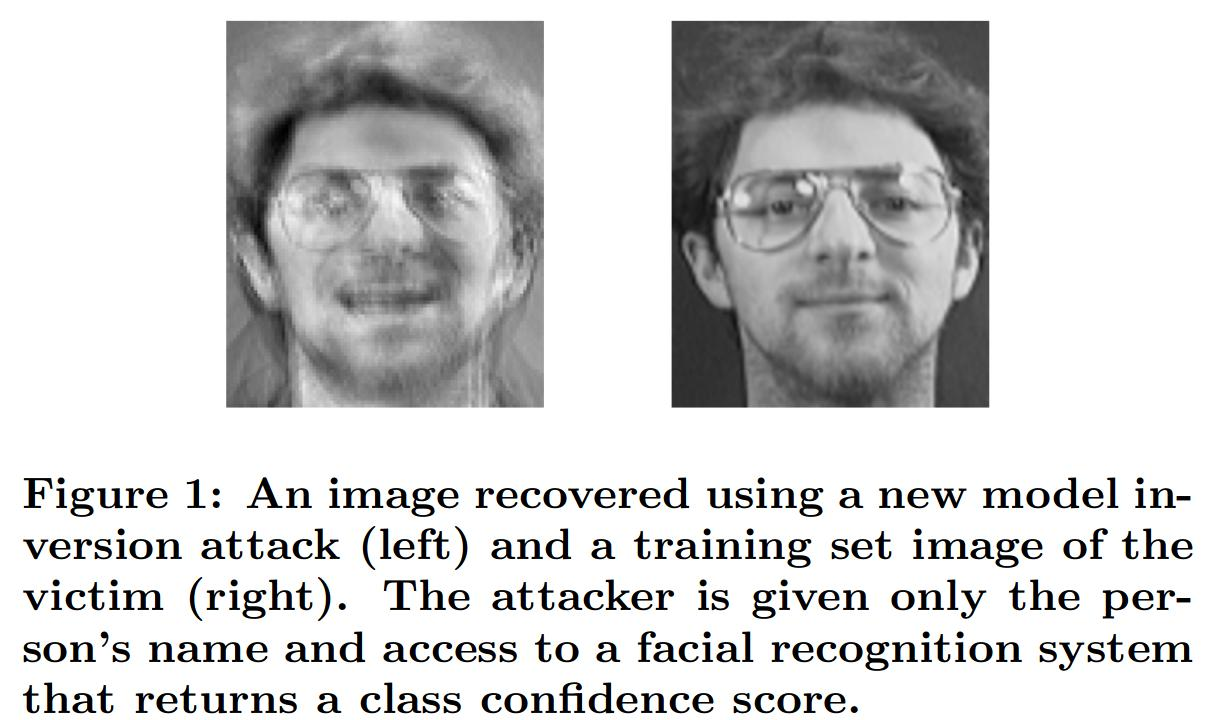
\includegraphics[width=0.6\linewidth]{img/fredrikson.et.al.jpg}

\begin{itemize}
\item exploit confidence values exposed by the APIs
\item attacker can produce a recognizable image of a person, given only API access to a facial recognition system and the name of the person whose face is recognized by it
\end{itemize}

\begin{tikzpicture}[overlay, remember picture]
\node at (current page.north east)[ref] {
\fullcite{Fredrikson.et.al.2015.SIGSAC} \par};
\end{tikzpicture}


\end{frame}


\section{Stochastic Gradient Descent recap}


\subsection{Finding the best model's parameters}


\begin{frame}{Training as optimization}
$$
\mathcal{L}(\Theta) = \frac{1}{n} \sum_{i =1}^{n} L (f(\bm{x}_i; \Theta), y_i)
$$

The training examples are fixed, and the values of the parameters determine the loss

The goal of the training algorithm is to set the values of the parameters $\Theta$‚ such that
the value of $\mathcal{L}$ is minimized
$$
\hat{\Theta} = \argmin_{\Theta} \mathcal{L}(\Theta) = \argmin_{\Theta} \frac{1}{n} \sum_{i =1}^{n} L (f(\bm{x}_i; \Theta), y_i)
$$


\end{frame}



\begin{frame}{(Online) Stochastic Gradient Descent}

\begin{algorithmic}[1]
	\Function{SGD}{$f(\bm{x}; \Theta)$, $(\bm{x}_1, \ldots, \bm{x}_n)$, $(\bm{y}_1, \ldots, \bm{y}_n)$, $L$}
	\While{stopping criteria not met}
		\State Sample a training example $\bm{x}_i, \bm{y}_i$
		\State Compute the loss $L(f(\bm{x}_i; \Theta), \bm{y}_i)$
		\State $\hat{\bm{g}} \gets$ gradient of $L(f(\bm{x}_i; \Theta), \bm{y}_i)$ wrt.\ $\Theta$
		\State $\Theta \gets \Theta - \eta_t \hat{\bm{g}}$
	\EndWhile
	\State \Return $\Theta$
	\EndFunction
\end{algorithmic}

Loss in line 4 is based on a \textbf{single training example} $\to$ a rough estimate of the corpus loss $\mathcal{L}$ we aim to minimize

The noise in the loss computation may result in inaccurate gradients

\end{frame}


\begin{frame}{Minibatch Stochastic Gradient Descent}
	
	\begin{algorithmic}[1]
		\Function{mbSGD}{$f(\bm{x}; \Theta)$, $(\bm{x}_1, \ldots, \bm{x}_n)$, $(\bm{y}_1, \ldots, \bm{y}_n)$, $L$}
		\While{stopping criteria not met}
		\State Sample $m$ examples $\{ (\bm{x}_1, \bm{y}_1), \ldots (\bm{x}_m, \bm{y}_m) \}$
		\State $\hat{\bm{g}} \gets 0$
		\For{$i = 1$ to $m$}
			\State Compute the loss $L(f(\bm{x}_i; \Theta), \bm{y}_i)$
			\State $\hat{\bm{g}} \gets \hat{\bm{g}}\ + $ gradient of $\frac{1}{m} L(f(\bm{x}_i; \Theta), \bm{y}_i)$ wrt.\ $\Theta$
		\EndFor
		\State $\Theta \gets \Theta - \eta_t \hat{\bm{g}}$
		\EndWhile
		\State \Return $\Theta$
		\EndFunction
	\end{algorithmic}
	

\end{frame}




\section{How to privatize SGD with DP}

\begin{frame}{What can we privatize in the SGD algorithm by DP?}

\begin{algorithmic}[1]
	\Function{SGD}{$f(\bm{x}; \Theta)$, $(\bm{x}_1, \ldots, \bm{x}_n)$, $(\bm{y}_1, \ldots, \bm{y}_n)$, $L$}
	\While{stopping criteria not met}
		\State Sample a training example $\bm{x}_i, \bm{y}_i$
		\State Compute the loss $L(f(\bm{x}_i; \Theta), \bm{y}_i)$
		\State $\hat{\bm{g}} \gets$ gradient of $L(f(\bm{x}_i; \Theta), \bm{y}_i)$ wrt.\ $\Theta$
		\State $\Theta \gets \Theta - \eta_t \hat{\bm{g}}$
	\EndWhile
	\State \Return $\Theta$
	\EndFunction
\end{algorithmic}

\pause
\begin{itemize}
\item Privatize input
\item Privatize output
\item Privatize learning
\end{itemize}

\end{frame}

\subsection{Problem 1: Unbounded gradient and unbounded sensitivity}

\begin{frame}{Unbounded sensitivity of gradient}

\begin{block}{Standard SGD}
\begin{algorithmic}[1]
\State $\ldots$
\State $\bm{g}(\bm{x}_i) \gets \nabla \mathcal{L} (\theta_t, \bm{x}_i)$
\Comment{Compute gradient}
\State $\ldots$
\end{algorithmic}
\end{block}


Clip the gradient vector by \textbf{per-example} $\ell_2$ norm
$$
\begin{aligned}
\bm{g}(\bm{x}_i) &\gets \nabla \mathcal{L} (\theta_t, \bm{x}_i) \\
\bar{\bm{g}}(\bm{x}_i) &\gets
\frac{
\bm{g}(\bm{x}_i)
}{
\max \left(1,
\frac{\norm{\bm{g}(\bm{x}_i)}_2}{C} \right)
}
\end{aligned}
$$
where $C \in \mathbb{R}$ is a clipping constant (hyper-parameter)




\end{frame}


\subsection{Problem 2: Too many steps for simple composition}

\begin{frame}{Running several mechanisms on the same data}

\begin{algorithmic}[1]
	\Function{SGD}{$f(\bm{x}; \Theta)$, $(\bm{x}_1, \ldots, \bm{x}_n)$, $(\bm{y}_1, \ldots, \bm{y}_n)$, $L$}
	\While{stopping criteria not met}
		\State $\ldots$
	\EndWhile
	\State \Return $\Theta$
	\EndFunction
\end{algorithmic}

Composition theorems: Running the same or various privacy mechanisms on the same data

\begin{block}{Basic composition --- ``epsilons and deltas add up"}
For $k \in \mathbb{N}$, the composition of $k$ mechanisms (each of them is $(\varepsilon, \delta)$-DP) gives $(k \varepsilon, k \delta)$-DP
\end{block}

This would lead to an excessively high overall budget

\end{frame}


\begin{frame}{Running several mechanisms on the same data}

\begin{block}{Basic composition --- ``epsilons and deltas add up"}
For $k$ steps (each $(\varepsilon, \delta)$-DP): $(k \varepsilon, k \delta)$-DP
\end{block}

$k$-fold adaptive composition of an $(\varepsilon, \delta)$-DP mechanism
	
\begin{block}{Advanced composition --- using smaller overall budget}
For $\delta' > 0$ and
$\varepsilon' = \varepsilon \sqrt{2 k \ln( 1 / \delta')} + k \varepsilon ( \exp(\varepsilon) - 1)$
the composite mechanism is $(\varepsilon', k \delta + \delta')$-DP
\end{block}

Great news: Advanced composition gives us quadratic improvement wrt.\ number of steps $k$
\begin{itemize}
\item $\approx \sqrt{k} \cdot \varepsilon$ instead of simple $k \cdot \varepsilon$
\end{itemize}

\begin{tikzpicture}[overlay, remember picture]
\node at (current page.north east)[ref] {
Theorem III.3 in \fullcite{Dwork.et.al.2010.FOCS} \par};
\end{tikzpicture}


\end{frame}

\subsection{Trick 3: Sub-sampling helps to reduce the budget in each step}


\begin{frame}{Privacy amplification by sub-sampling}

Let's define a \textbf{sampling function} that takes a dataset $D_{\mathrm{in}} \in \mathcal{X}$ and produces another dataset $D_{\mathrm{out}} \in \mathcal{X}$ as follows:

\begin{itemize}
\item For each entry $t$ from $D_{\mathrm{in}}$ the function draws a binary value at random
\begin{itemize}
\item We draw `zero or one' using a Bernoulli random variable $\mathrm{Ber}(\beta)$ parametrized by $\beta \in (0, 1)$
\end{itemize}
\item If it's $1$, this entry $t$ will end up in the output dataset $D_{\mathrm{out}}$
\item If it's $0$, this entry is ignored
\end{itemize}

\textbf{Important:} For each entry $t$ the Bernoulli trial is independent of other entries

This is also known as \textbf{Poisson sampling}

\end{frame}

\begin{frame}{Privacy amplification by sub-sampling}

Let's have an $(\varepsilon_1, \delta_1)$-DP algorithm $\mathcal{A}_1$

We propose a new algorithm $\mathcal{A}_2$ that works in two steps:
\begin{enumerate}
\item Sub-sample our dataset $D$ using Poisson sampling (with parameter $\beta$)
\item Run $\mathcal{A}_1$ on this smaller dataset
\end{enumerate}

Then $\mathcal{A}_2$ is $(\varepsilon_2, \delta_2)$-DP, where
$$
\varepsilon_2 = \ln \left(
1 + \beta \left[
\exp(\varepsilon_1) - 1 \right]
\right)
\qquad
\delta_2 = \beta \delta_1
$$

\begin{tikzpicture}[overlay, remember picture]
\node at (current page.north east)[ref] {
Proof in the appendix of \fullcite{Li.et.al.2012.ASIACCS}; there are a few `nasty' typos. \par};
\end{tikzpicture}


\end{frame}


\begin{frame}{How much we can `save' on the privacy budget?}

\begin{figure}
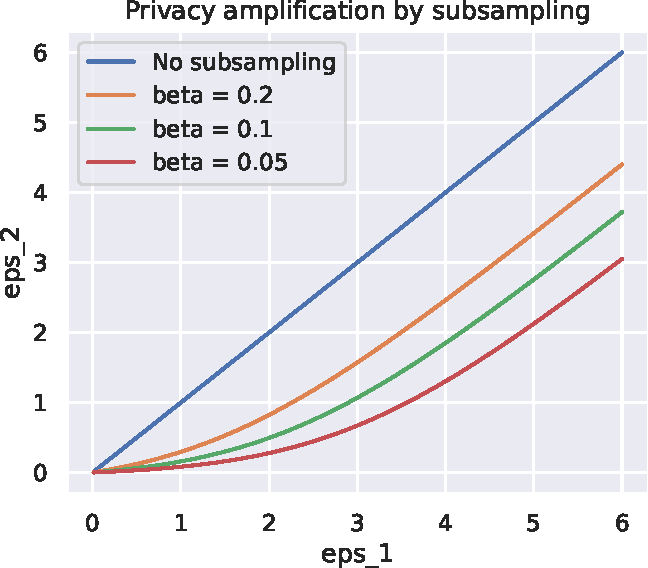
\includegraphics[width=0.7\linewidth]{img/privacy-amplification-01.pdf}
\end{figure}


\end{frame}



\begin{frame}{Why is Poisson sampling relevant for SGD?}

Recall Mini-batch SGD!

\begin{algorithmic}[1]
\Function{mbSGD}{$f(\bm{x}; \Theta)$, $(\bm{x}_1, \ldots, \bm{x}_n)$, $(\bm{y}_1, \ldots, \bm{y}_n)$, $L$}
\While{stopping criteria not met}
\State Sample $m$ examples $\{ (\bm{x}_1, \bm{y}_1), \ldots (\bm{x}_m, \bm{y}_m) \}$
\State $\ldots$
\EndWhile
\EndFunction
\end{algorithmic}


\begin{itemize}
\item We usually use small `batches' which are somehow randomly subsampled from the training dataset
\item We can replace the minibatch sampling with Poisson sampling!
\end{itemize}


\end{frame}


\section{DP-SGD}


\begin{frame}{DP-SGD algorithm}
	
\begin{minipage}[t][10cm][t]{15cm}

\begin{algorithmic}[1]
\Function{DP-SGD}{$f(\bm{x}; \Theta)$, $(\bm{x}_1, \ldots, \bm{x}_n)$, $|L|$ --- `lot' size, $T$ --- \# of steps}
\For{$t \in (1, 2, \ldots, T)$}
\State Add each training example to a `lot' $L_t$ with probability $|L|/n$
\For{each example in the `lot' $\bm{x}_i \in L_t$}
\State $\bm{g}(\bm{x}_i) \gets \nabla \mathcal{L} (\theta_t, \bm{x}_i)$
\Comment{Compute gradient}
\State
$\bar{\bm{g}}(\bm{x}_i) \gets \bm{g}(\bm{x}_i) / \max \left(1 , \|  \bm{g}(\bm{x}_i) \| / C \right)
$
\Comment{Clip gradient}
\State $\tilde{\bm{g}}(\bm{x}_i) \gets \bar{\bm{g}}(\bm{x}_i) + \mathcal{N}(0, \sigma^2 C^2 \bm{I})$
\Comment{Add noise}
\EndFor
\State $\hat{\bm{g}} \gets \frac{1}{|L|} \sum_{k = 1}^{|L|} \tilde{\bm{g}}(\bm{x}_k)$
\Comment{Gradient estimate of `lot' by averaging}
\State $\Theta_{t + 1} \gets \Theta_t - \eta_t \hat{\bm{g}}$
\Comment{Update parameters by gradient descend}
\EndFor
\State \Return $\Theta$
\EndFunction
\end{algorithmic}

\end{minipage}
	
\end{frame}



\begin{frame}{Stochastic gradient descent with differential privacy}

Setup: A set of labeled i.i.d.\ examples --- like tabular data (each example = single person)

Privacy `accountant' --- utilizes composition of DP
\begin{itemize}
	\item Computes the privacy cost at each access to the training data (gradient computation)
	\item Accumulates this cost as the training progresses
\end{itemize}

Tightest privacy by numerical integration to get bounds on the \textbf{moment generating function} of the \textbf{privacy loss random variable} for all moments $\leq 32$

\begin{tikzpicture}[overlay, remember picture]
\node at (current page.north east)[ref] {
\fullcite{Abadi.et.al.2016.SIGSAC} \par};
\end{tikzpicture}

\end{frame}



\begin{frame}{Recap of DP-SGD}

\begin{itemize}
\item DP-SGD `de-facto' standard for supervised training with DP
\item Implemented in Opacus, Tensorflow privacy, and other libs
\end{itemize}

What makes it tricky?

\begin{itemize}
\item Remember: Data points \textbf{must} be independent (privacy-wise)
\item Scalability: Per-example gradient norm and clipping is super slow
\end{itemize}


\begin{tikzpicture}[overlay, remember picture]
\node at (current page.north east)[ref] {
\fullcite{Abadi.et.al.2016.SIGSAC} \par};
\end{tikzpicture}

\end{frame}


\section{The Obvious Application: Supervised Training}

\begin{frame}{DP-SGD across various NLP tasks}

Setup:

Although DP-SGD had been used in language modeling, the community lacked a thorough understanding of its usability across different NLP tasks

Research questions:

\begin{itemize}
\item Which models and training strategies provide the best trade-off between privacy and performance on different NLP tasks?
\item How exactly do increasing privacy requirements hurt the performance?
\end{itemize}


\begin{tikzpicture}[overlay, remember picture]
\node at (current page.north east)[ref] {
\fullcite{senge-etal-2022-one} \par};
\end{tikzpicture}

\end{frame}


\begin{frame}{DP-SGD across various NLP tasks: Datasets}



\begin{table}
\scriptsize
\begin{tabular}{llrr}
\toprule
{Task} & {Dataset} & {Size} & {Classes}\\ 
\hline
SA & IMDb & 50k documents & 2\\
NLI&  SNLI &  570k pairs &  3\vspace{0.7em}\\
NER &  CoNLL'03 &  $\approx$ 300k tokens &  9 \\
NER & Wikiann & $\approx$ 320k tokens & 7\\
POS & GUM & $\approx$ 150k tokens  & 17 \\
POS & EWT & $\approx$ 254k tokens & 17\vspace{0.7em}\\
QA&  SQuAD 2.0 & 150k questions  &  $\star$ \\
\bottomrule
\end{tabular}
\caption{Datasets and their specifics. $\star$ SQuAD contains 100k answerable and 50k unanswerable questions, where answerable questions are expressed as the span positions of their answer.}
\label{tab:dataset}
\end{table}



\begin{tikzpicture}[overlay, remember picture]
\node at (current page.north east)[ref] {
\fullcite{senge-etal-2022-one} \par};
\end{tikzpicture}

\end{frame}


\begin{frame}{DP-SGD across various NLP tasks: Results}


\begin{figure}
	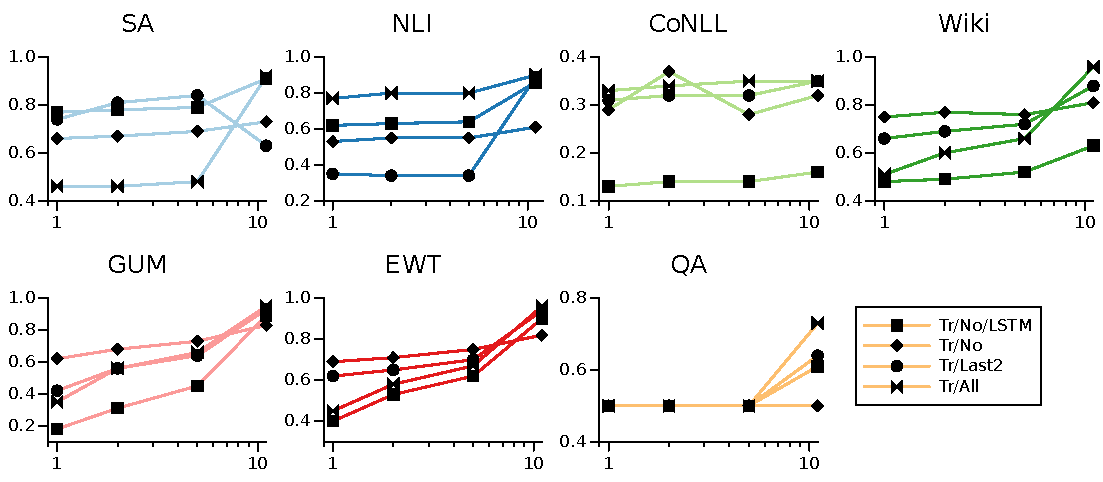
\includegraphics[width=\linewidth]{img/plot-fig2.pdf}
	\caption{\label{fig:performance-by-task} Comparison of BERT performances (macro $F_1$ score) per dataset with varying privacy budget $\varepsilon \in \{1, 2, 5, \infty \}$ on the $x$-axis (note the $\log$ scale).}
\end{figure}


\begin{tikzpicture}[overlay, remember picture]
\node at (current page.north east)[ref] {
\fullcite{senge-etal-2022-one} \par};
\end{tikzpicture}

\end{frame}



\section{The Less Obvious Application: Language Models}

\begin{frame}{Early DP language models}

Motivated by the problem of training models for next-word prediction in a mobile keyboard; used this as a running example

\begin{tikzpicture}[overlay, remember picture]
\node at (current page.north east)[ref] {
\fullcite{McMahan.et.al.2018.ICLR} \par};
\end{tikzpicture}

\end{frame}

\begin{frame}{Early DP language models: Neighboring datasets}

Most prior work on differentially private machine learning deals with example-level privacy

--- Two datasets $D$ and $D'$ are defined to be adjacent if $D'$ can be formed by adding or removing a \textbf{single training example} from $D$

But:

--- A sensitive word or phrase may be typed several times by an individual user, but it should still be protected

\begin{tikzpicture}[overlay, remember picture]
\node at (current page.north east)[ref] {
\fullcite{McMahan.et.al.2018.ICLR} \par};
\end{tikzpicture}

\end{frame}

\begin{frame}{Early DP language models: Neighboring datasets}

\citet{McMahan.et.al.2018.ICLR} thus \textbf{defined}:

\begin{block}{Definition: User-adjacent datasets}
\small
Let $D$ and $D'$ be two datasets of training examples, where each example is associated with a user. Then, $D$ and $D'$ are adjacent if $D'$ can be formed by adding or removing \textbf{all of the examples associated with a single user} from $D$.
\end{block}

$D$ contains training examples, each associated with a user, e.g., $D = \{A_1, A_2, B_1, B_2\}$ where $\{A, B\}$ are the users. Then $D'$ can be formed by adding or removing all examples from one user, e.g., $D' = \{A_1, A_2\}$, or $D' = \{A_1, A_2, B_1, B_2, C_1\}$, but not $\{A_1, A_2, B_1\}$


\begin{tikzpicture}[overlay, remember picture]
\node at (current page.north east)[ref] {
\fullcite{McMahan.et.al.2018.ICLR} \par};
\end{tikzpicture}

\end{frame}


\begin{frame}{Early DP language models: Training the model with DP}

Their private algorithm relies heavily on two prior works
\begin{itemize}
\item FederatedAveraging (or FedAvg) algorithm of McMahan et al. (2016), which trains deep networks on user-partitioned data
\item the moments accountant of Abadi et al. (2016), which provides tight composition guarantees for the repeated application of the Gaussian mechanism combined with amplification-via-sampling
\end{itemize}

\begin{tikzpicture}[overlay, remember picture]
\node at (current page.north east)[ref] {
\fullcite{McMahan.et.al.2016.arXiv} \par};
\end{tikzpicture}

\end{frame}


\begin{frame}{Early DP language models: Training the model with DP}

FedAvg was introduced by McMahan et al. (2016) for federated learning, where the goal is to train a shared model while leaving the training data on each user’s mobile device. Instead, devices download the current model and compute an update by performing local computation on their dataset.

Most importantly, the algorithm naturally forms per-user updates based on a single user’s data, and these updates are then averaged to compute the final update applied to the shared model on each round.

This structure makes it possible to extend the algorithm to provide a user-level differential privacy guarantee.

\begin{tikzpicture}[overlay, remember picture]
\node at (current page.north east)[ref] {
\fullcite{McMahan.et.al.2016.arXiv} \par};
\end{tikzpicture}

\end{frame}


\begin{frame}{Early DP language models: Training the model with DP}

To achieve differential privacy:

\begin{itemize}
\item A) They use random-sized batches where we select users independently with probability $q$, rather than always selecting a fixed number of users.
\item B) They enforce clipping of per-user updates so the total update has bounded $\ell_2$ norm.
\item C) (They use different estimators for the average update)
\item D) They add Gaussian noise to the final average update.
\end{itemize}


\begin{tikzpicture}[overlay, remember picture]
\node at (current page.north east)[ref] {
\fullcite{McMahan.et.al.2018.ICLR} \par};
\end{tikzpicture}

\end{frame}


\begin{frame}{Early DP language models: Data and evaluation}

\begin{block}{Data}
\small
Used a large public dataset of Reddit posts

Each post in the database is keyed by an author, so they group the data by these keys in order to provide user-level privacy.

763,430 users each with 1600 tokens
\end{block}

\begin{block}{Evaluation}
\small
-- LSTM language model (1.35M params)

-- They evaluate using \texttt{AccuracyTop1}, the probability that the word to which the model assigns highest probability is correct
\end{block}

\begin{tikzpicture}[overlay, remember picture]
\node at (current page.north east)[ref] {
\fullcite{McMahan.et.al.2018.ICLR} \par};
\end{tikzpicture}

\end{frame}

\begin{frame}{Early DP language models: Results}

\begin{figure}
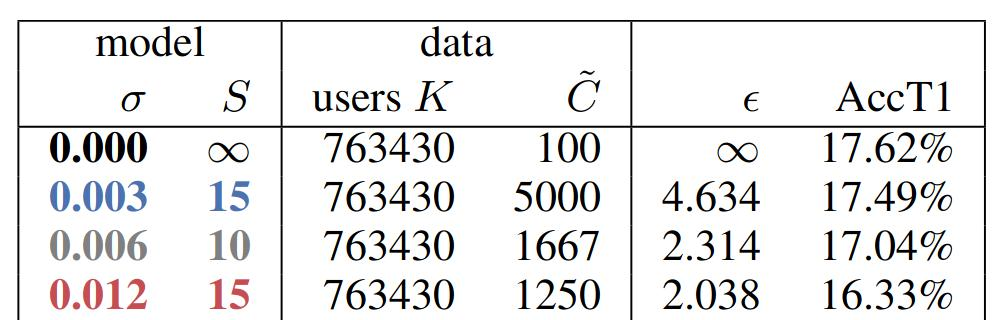
\includegraphics[width=0.8\linewidth]{img/mcmahan-table1.jpg}
\end{figure}

\begin{tikzpicture}[overlay, remember picture]
\node at (current page.north east)[ref] {
\fullcite{McMahan.et.al.2018.ICLR} \par};
\end{tikzpicture}

\end{frame}


\section{When Things Go Tricky}


\begin{frame}{Poisson subsampling versus just batches?}

The `standard' random shuffling method for iterating over batches providing a weaker privacy guarantee for the training data than Poisson sampling.

--- Experiments with Neural Machine Translation


\begin{tikzpicture}[overlay, remember picture]
\node at (current page.north east)[ref] {
\fullcite{igamberdiev-etal-2024-dp} \par};
\end{tikzpicture}

\end{frame}


\begin{frame}{Datasets}

--- WMT-16 (DE-EN) language pair

--- Business Scene Dialogue corpus (BSD), a collection of fictional business conversations in various scenarios (e.g. “face-to-face”, “phone call”, “meeting”), Japanese and English

--- ClinSPEn-CC, a collection of parallel COVID-19 clinical cases in English and Spanish


\begin{table}
\scriptsize
\begin{tabular}{lr|rr}
\textbf{Dataset} & \textbf{Lang. Pair} & \textbf{\texttt{\#} Trn.+Vld.} & \textbf{\texttt{\#} Test} \\
\hline
WMT-16 & DE-EN & 4,551,054 & 2,999 \\
BSD & JA-EN & 22,051 & 2,120 \\
ClinSPEn-CC & ES-EN & 1,065 & 2,870 \\  % 968 + 97
\end{tabular}
\end{table}


\begin{tikzpicture}[overlay, remember picture]
\node at (current page.north east)[ref] {
\fullcite{igamberdiev-etal-2024-dp} \par};
\end{tikzpicture}

\end{frame}


\begin{frame}{Results}

\begin{figure}
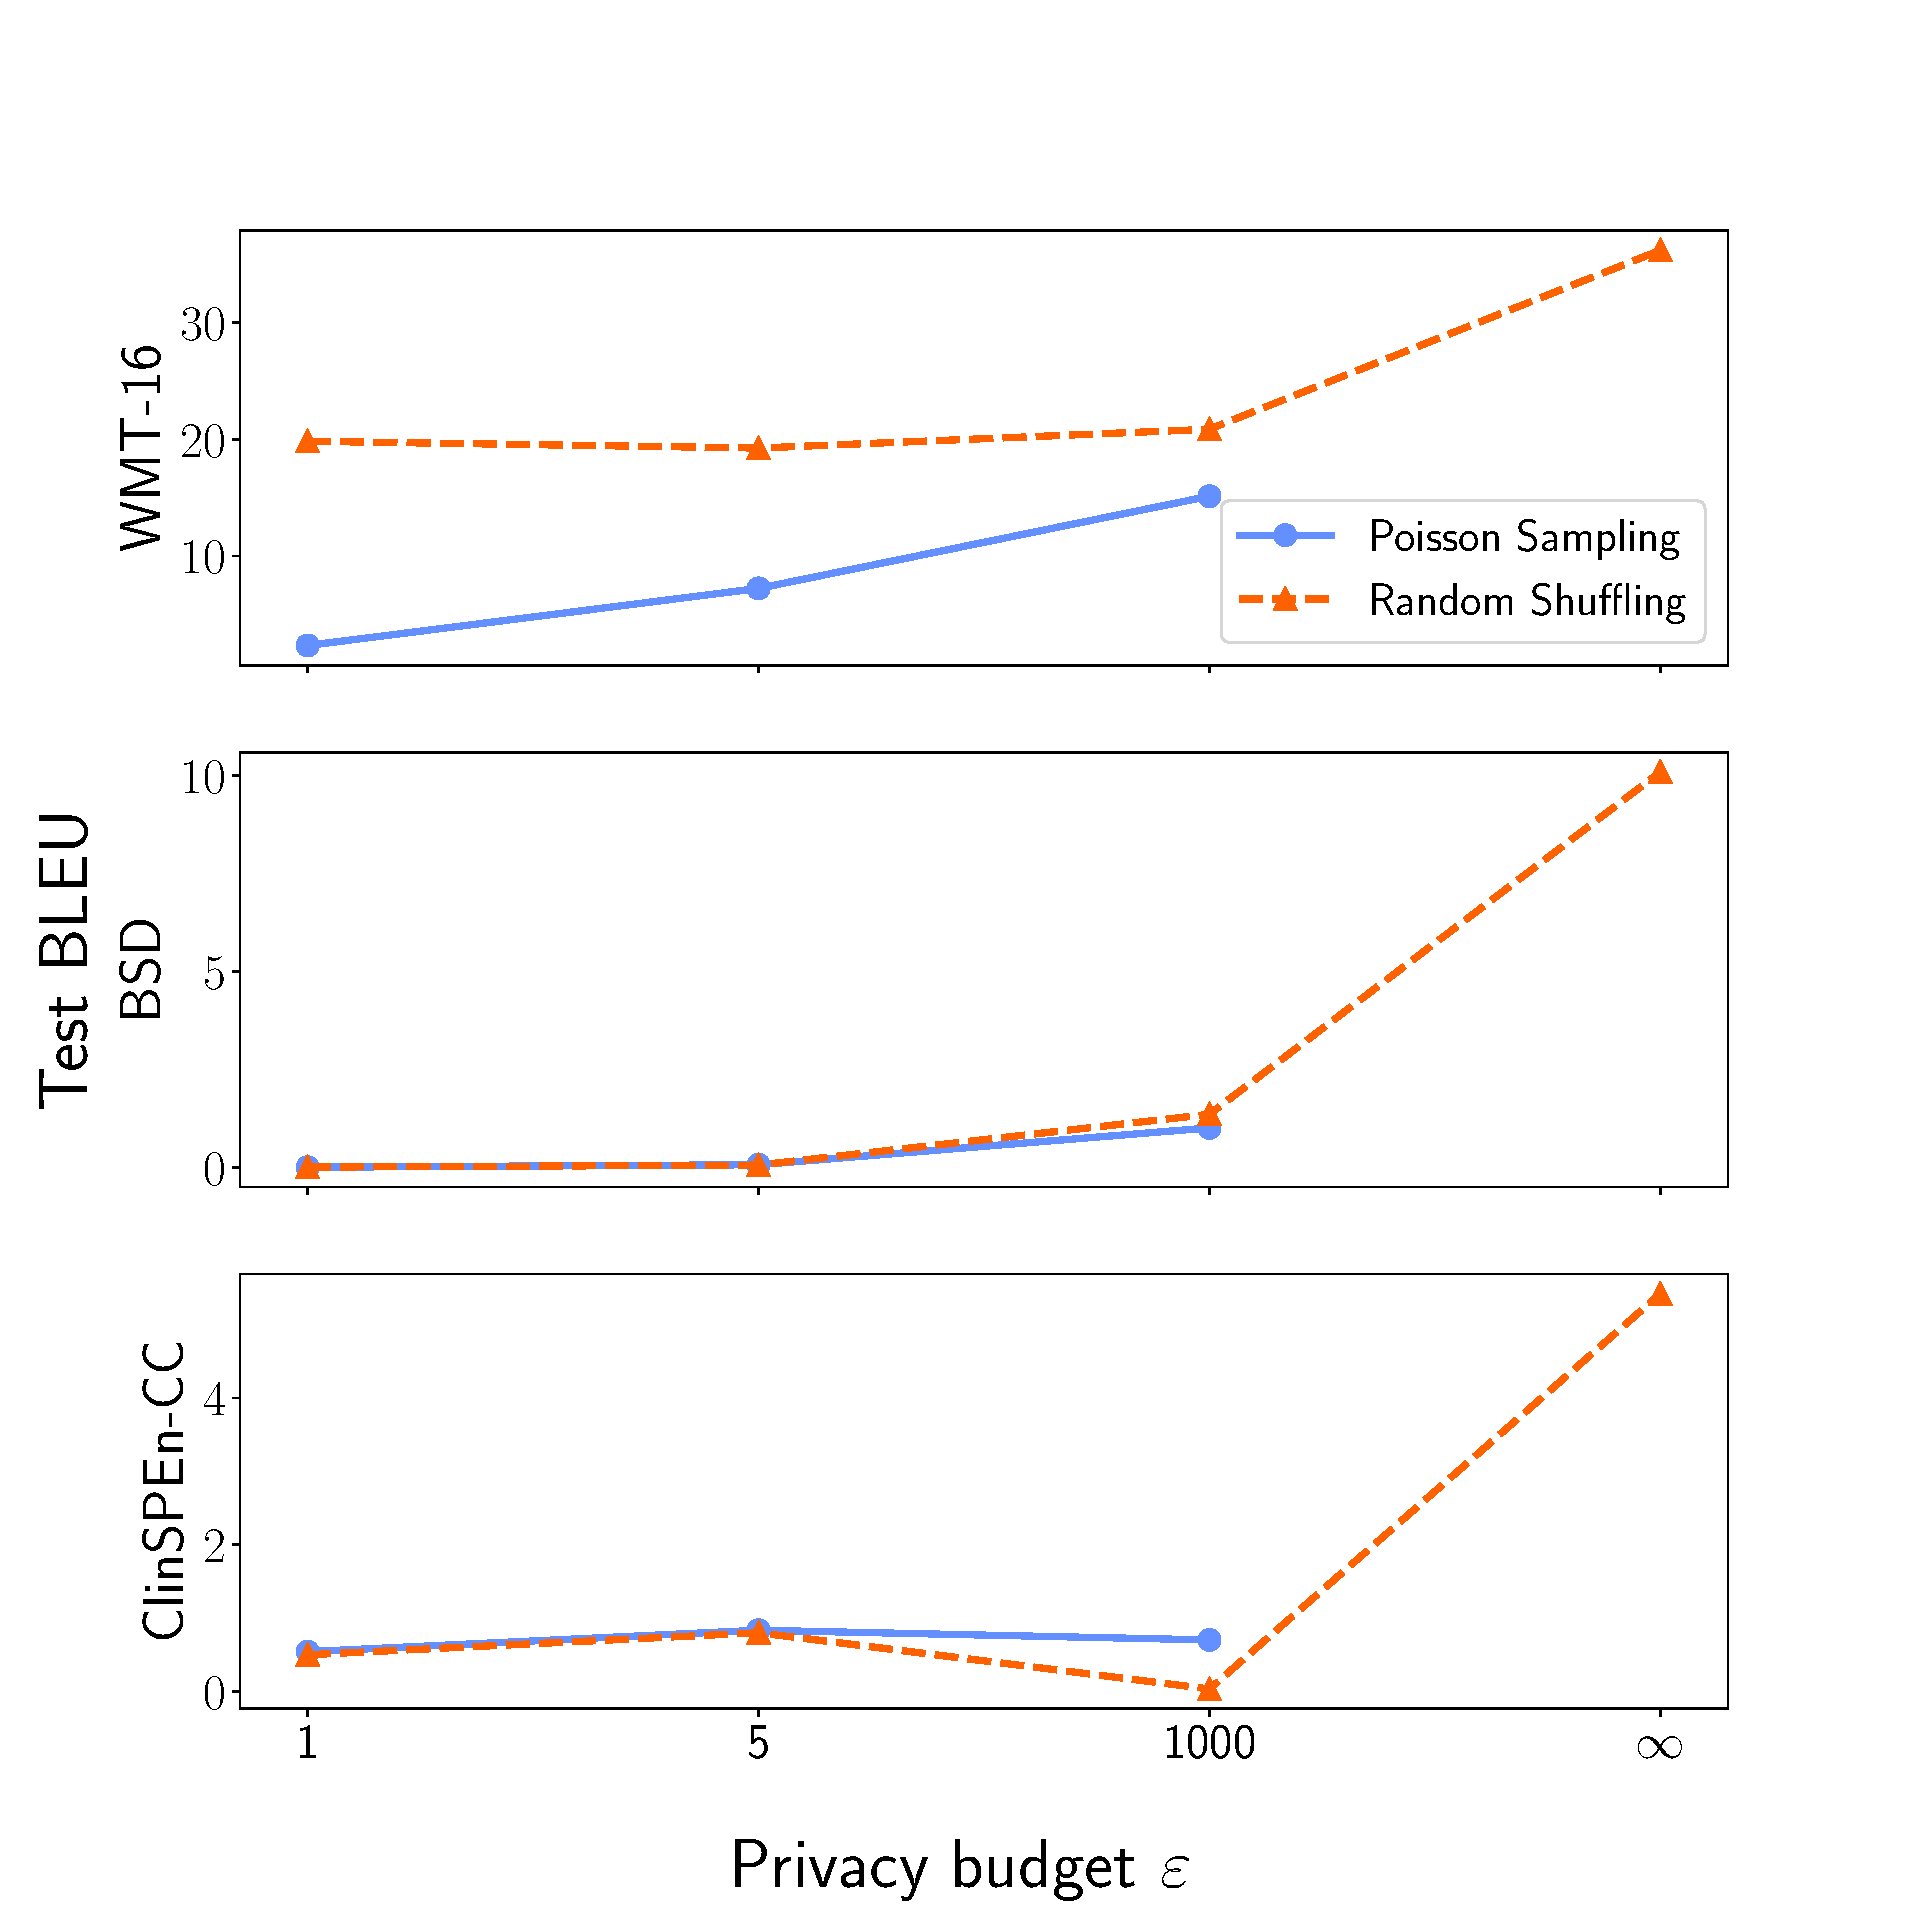
\includegraphics[trim={0 0 3cm 3.5cm},clip,width=0.6\linewidth]{img/results-test-BLEU.pdf}
\end{figure}

\begin{tikzpicture}[overlay, remember picture]
\node at (current page.north east)[ref] {
\fullcite{igamberdiev-etal-2024-dp} \par};
\end{tikzpicture}

\end{frame}



\section{When Things Go Very Tricky}


\begin{frame}{Private information in text?}


our understanding of what is \textit{private information} in textual data is still very limited

Applications of DP --- guarantee to each individual \textit{data point}

For textual data, a single data point will often be a sentence or document.

However, this does not mean that there is a one-to-one mapping from \textit{individuals} to sentences and documents.
For instance, multiple documents could potentially refer to the same individual, or contain the same piece of sensitive information that would break the assumption of each data point being independent.

\begin{tikzpicture}[overlay, remember picture]
\node at (current page.north east)[ref] {
\fullcite{igamberdiev-etal-2024-dp} \par};
\end{tikzpicture}

\end{frame}


\begin{frame}{Private information in text?}


``In this paper, we discuss the mismatch between the narrow assumptions made by popular data protection techniques (data sanitization and differential privacy), and the broadness of natural language and of privacy as a social norm.''


``We argue that existing protection methods cannot guarantee a generic and meaningful notion of privacy for language models. We conclude that language models should be trained on text data which was explicitly produced for public use."

\begin{tikzpicture}[overlay, remember picture]
\node at (current page.north east)[ref] {
\fullcite{Brown.et.al.2022.FAcT} \par};
\end{tikzpicture}

\end{frame}



\begin{frame}{Private information in text?}

The approach to preserving privacy in LMs has been to attempt complete removal of private information from training data (data sanitization), or to design algorithms that do not memorize private data, such as algorithms that satisfy differential privacy (DP)

Both methods make explicit and implicit assumptions about the structure of data to be protected, the nature of private information, and requirements for privacy, that do not hold for the majority of natural language data.

\begin{tikzpicture}[overlay, remember picture]
\node at (current page.north east)[ref] {
\fullcite{Brown.et.al.2022.FAcT} \par};
\end{tikzpicture}

\end{frame}



\begin{frame}{Private information in text?}

\begin{figure}
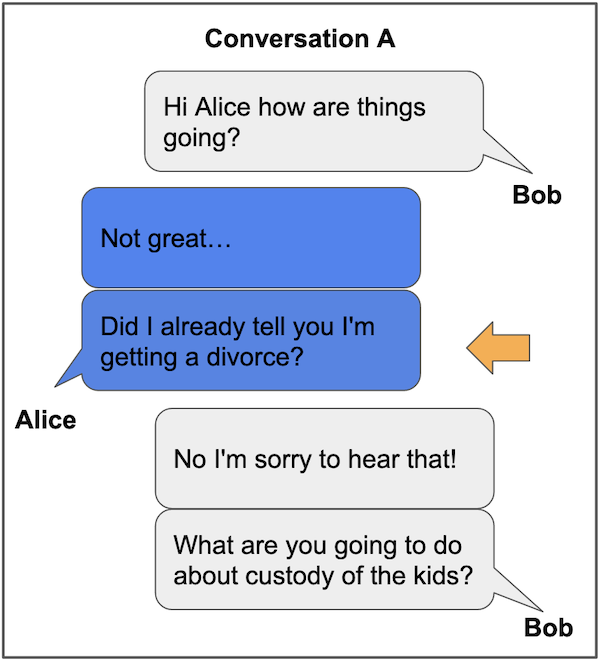
\includegraphics[width=0.45\linewidth]{img/out1.png}
\caption{Original conversation. Private information indicated by orange arrows.}
\end{figure}


\begin{tikzpicture}[overlay, remember picture]
\node at (current page.north east)[ref] {
\fullcite{Brown.et.al.2022.FAcT} \par};
\end{tikzpicture}

\end{frame}


\begin{frame}{Private information in text?}

\begin{figure}
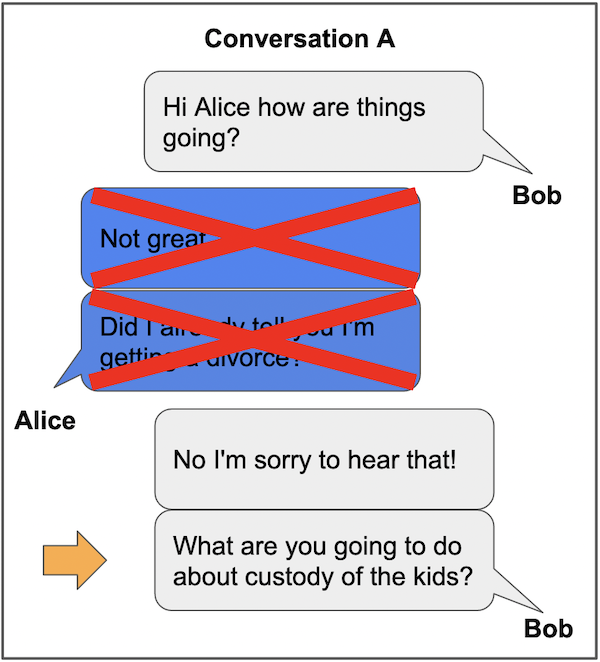
\includegraphics[width=0.45\linewidth]{img/out2.png}
\caption{Alice's messages removed. Bob's last message still includes her private information.}
\end{figure}


\begin{tikzpicture}[overlay, remember picture]
\node at (current page.north east)[ref] {
\fullcite{Brown.et.al.2022.FAcT} \par};
\end{tikzpicture}

\end{frame}


\begin{frame}{Private information in text?}

\begin{figure}
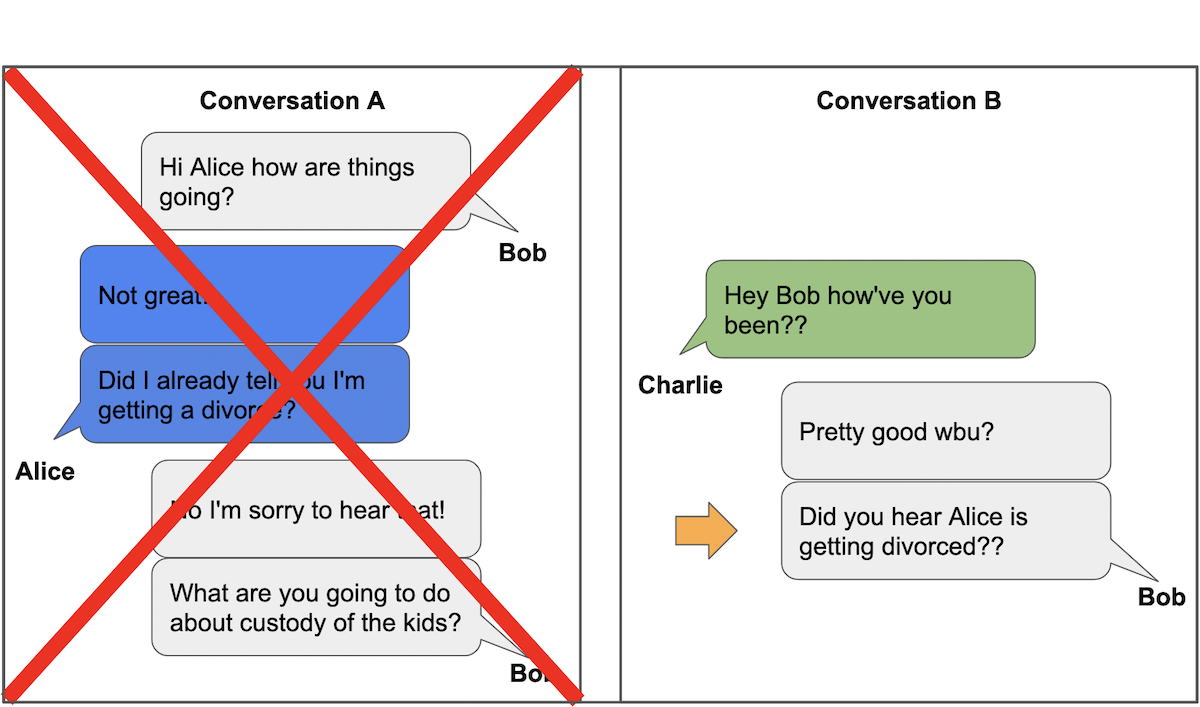
\includegraphics[width=0.75\linewidth]{img/out3.png}
\caption{The whole original conversation is removed. Conversation B still contains Alice's private information though she is not in the conversation.}
\end{figure}


\begin{tikzpicture}[overlay, remember picture]
\node at (current page.north east)[ref] {
\fullcite{Brown.et.al.2022.FAcT} \par};
\end{tikzpicture}

\end{frame}




\begin{frame}{License and credits}

	\begin{columns}
		\begin{column}{0.7\textwidth}
			Licensed under Creative Commons Attribution-ShareAlike 4.0 International (CC BY-SA 4.0)
		\end{column}
		\begin{column}{0.2\textwidth}
			
\includegraphics[width=0.9\linewidth]{img/cc-by-sa-icon.pdf}
		\end{column}
	\end{columns}
	
	\bigskip
	
	Credits
	
	\begin{scriptsize}
		
		Ivan Habernal
		
		Content from ACL Anthology papers licensed under CC-BY \url{https://www.aclweb.org/anthology}
		
		Partly inspired by lectures from Gautam Kamath
	
	\end{scriptsize}
	
\end{frame}



\end{document}

